

\section{Orbfiold Tutte Embeding}
In this section, I will get into details of my project on orbifold Tutte embedding. I explore two geometry background: Euclidean and hyperbolic. This section is organized as follows: I will first introduce the theoretical background. Then I will give details on my implementation.

\subsection{Theoretical Background}
\subsubsection{Tutte Embedding}
Tutte embedding is very famous in the field of parameterization, because it can generate bijective parameterization. Tutte embedding is based on the following theorem \cite{Tutte1963graph}:
\begin{theorem}\label{tutte-theorem}
Let $G = \left<V , E , F \right>$ be a 3-connected planar graph with boundary vertices $B \subset V$ defining a unique unbounded exterior face $f_e$ . Suppose $\partial f_e$ is embedded in the plane as a (not necessarily strictly) convex planar polygon, and each interior vertex is positioned in the plane as a strictly convex combination of its neighbors, then the straight-line drawing of $G$ with these vertex positions is an embedding. In addition, this embedding has strictly convex interior faces.
\end{theorem}
The embedding problem is the following full-rank linear system:
\begin{equation}
\begin{split}
\sum_{v_j \in \mathit{N}(v_i)} w_{ij}(z_j-z_i) &= 0,  &v_i \in V - B\\
z_i &= z_i^0, &v_i \in B\\
\end{split}
\label{eq:tutte}
\end{equation}
where $w > 0$.

\cite{Gortler:2006:DOM:1133946.1648437} generalized this algorithm to high genus surface, but spherical surface wasn't touched.

System \ref{eq:tutte} is equivalent to the following optimization problem:

\begin{equation}
\begin{split}
&\min_{\Phi}\ \ \   E(z) = \frac{1}{2}\sum_{(i,j)\in E} w_{ij} d(z_i, z_j)^2 \\
s.t \ \ \   &z_i = z_i^0, \ \ \ \ v_i \in B
\end{split}
\end{equation}

We will use this equivalence in hyperbolic background

\subsubsection{Orbifolds}
The orbifold is a generalization of the manifold. Formal definition for general orbifold is very abstract. We only focus on what we will use: 2-dimensional sphere-type orbifolds, that is, they have the topology of sphere. In the following context, we assume all orbifolds are of this kind.

In this project, we simply treat an orbifold as a seamlessly tiled plane by a basic tile. The transformations between copies are orientation-preserved isometries in their corresponding geometric backgrounds. Fix point of some isometry is called cones or singularities. And if two points is differed by an transformation between two copies, they are equivalent. The quotient plane by these equivalent relations are called orbifolds.

We know cones are rotation center of some isometries. So an orbifold is determined by cones and their rotation angles. Examples are shown in Fig.\ref{fig:tile}. We use Poincare disk as hyperbolic geometry model.

\begin{figure}
\centering
\begin{subfigure}{0.5\textwidth}
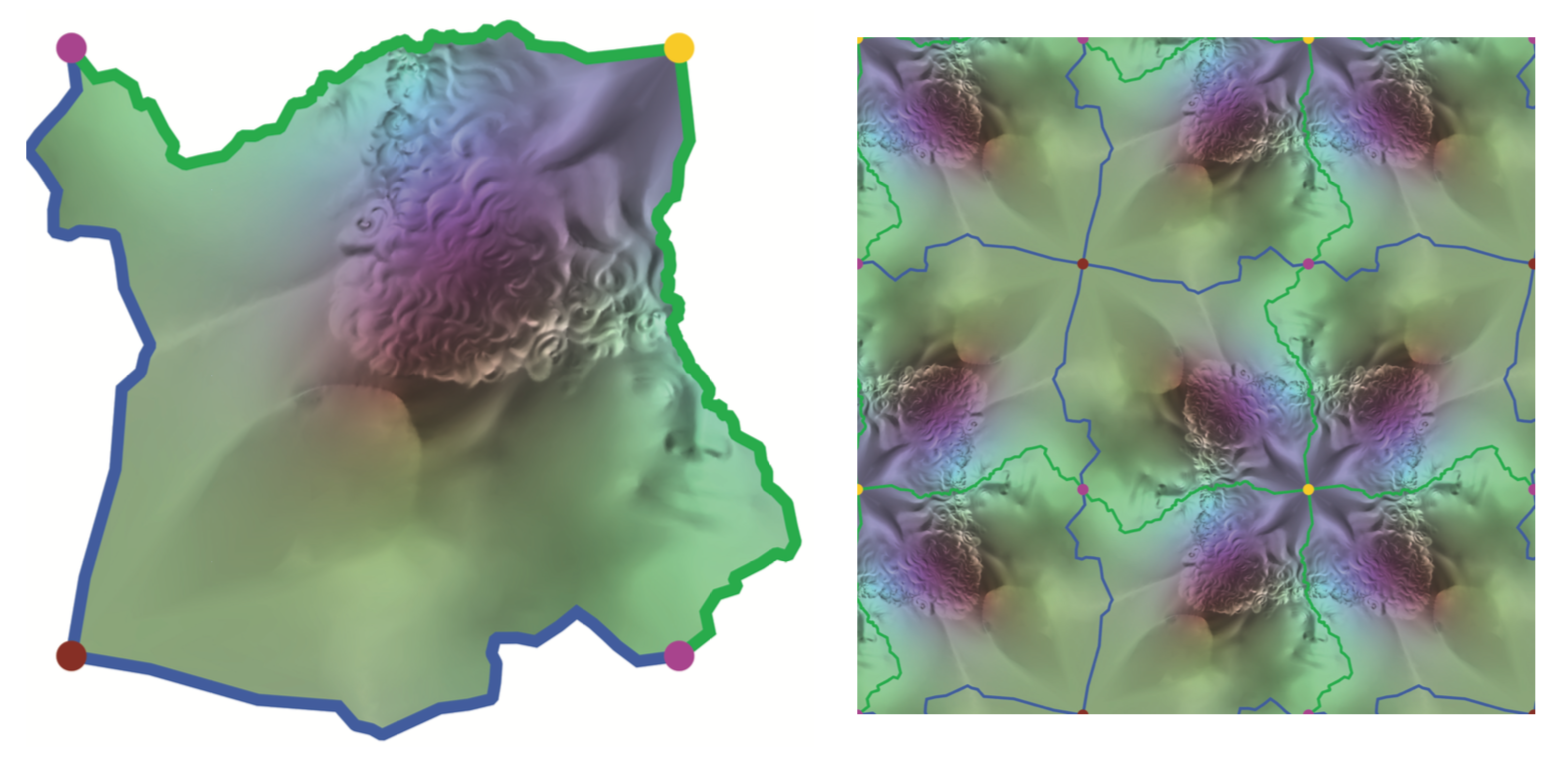
\includegraphics[width=\textwidth]{images/euc_orbifold}
\caption{}
\end{subfigure}
\begin{subfigure}{0.4\textwidth}
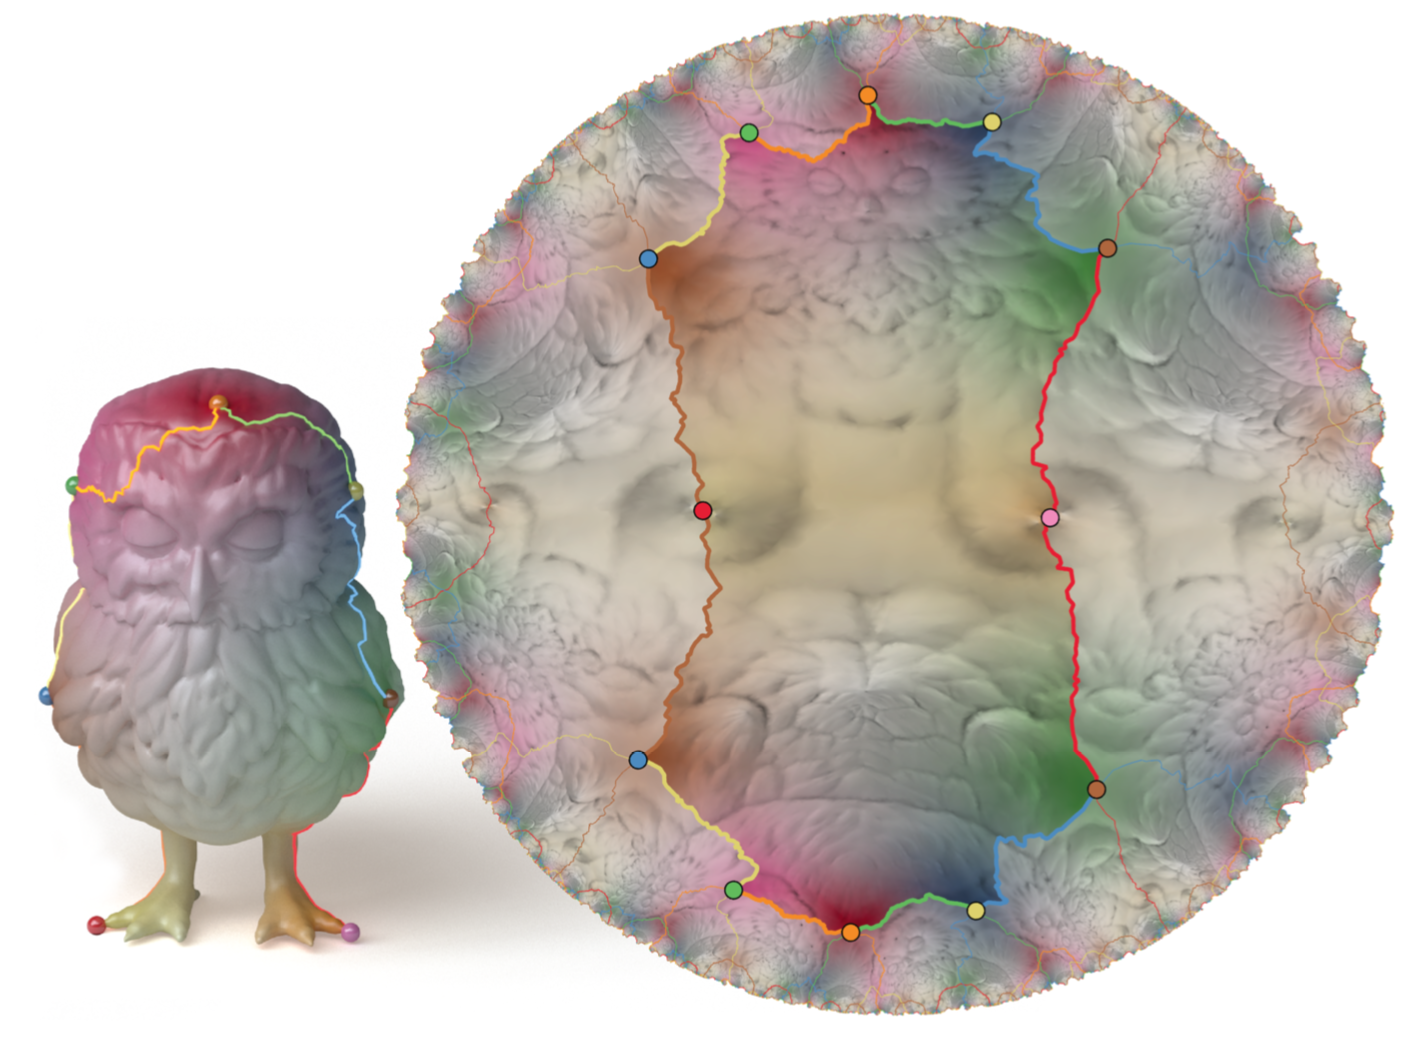
\includegraphics[width = \textwidth]{images/hyperbolic}
\caption{}
\label{fig:hyper-orbifold}
\end{subfigure}
\caption{(a) A Euclidean orbfold. (b) A hyperbolic orbifold.}
\label{fig:tile}
\end{figure}

\subsection{Algorithm}

The purpose of \cite{Aigerman:2015:OTE:2816795.2818099}\cite{Aigerman:2016:HOT:2980179.2982412} is generalize Tutte embedding onto sphere-type surfaces.

The algorithm is as follows:

1) Choose some cone set $C$, and find a path through all of them, cut the mesh $M$ into a disk type mesh $\bar{M}$.

2) Embed cones of $\bar{M}$ to some basic tile.

3) Solve the orbifold system.

In step 1, some of cones in the original mesh will be splitted into two copies. They are both cones in cutted mesh. 

In step 2, the positions of cones should satisfy the requirement of some orbifold. There are only four Euclidean orbifolds, shown in Fig.\ref{fig:four-kinds}. And for hyperbolic background, there are infinitely many. We simply set all cone angles be $\pi$, the method to compute the positions of cones are in the appendix of \cite{Aigerman:2016:HOT:2980179.2982412}

In step 3, we solve Tutte embedding system with orbifold constraints.

For Euclidean orbifolds, we solve the following linear system.

\begin{figure}
\centering
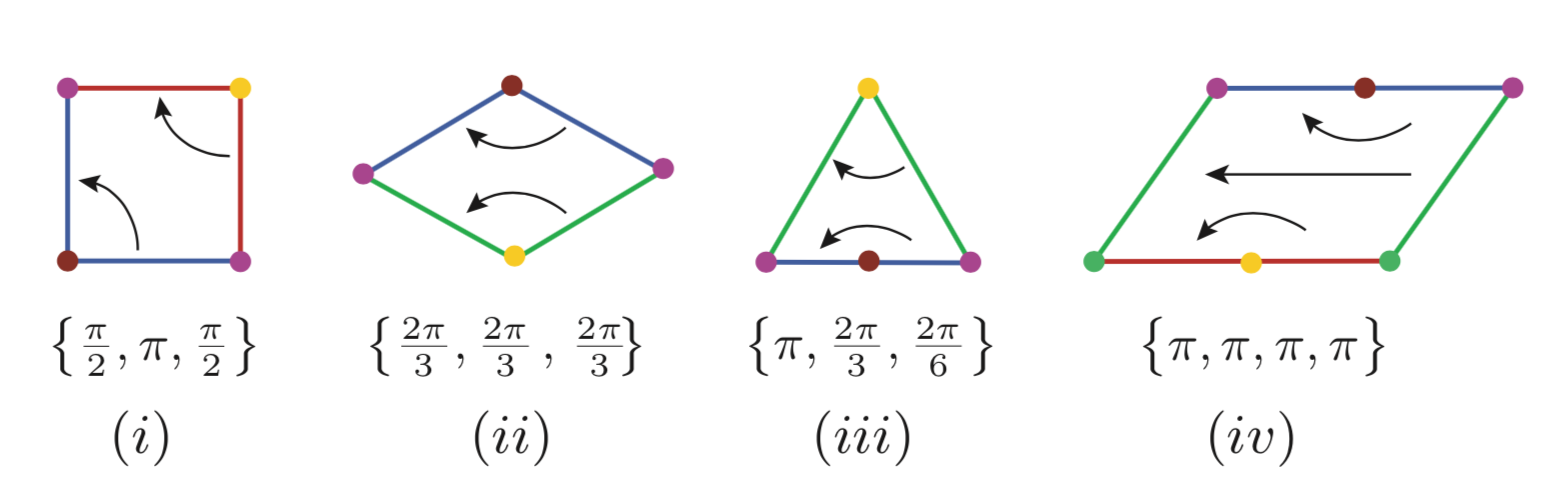
\includegraphics[width=0.5\textwidth]{images/four_euc_orbifolds}
\caption{Four kinds of sphere-type Euclidean orbifolds}
\label{fig:four-kinds}
\end{figure}

\begin{equation}
\begin{split}
\sum_{v_j \in N(v_i)}w_{ij}(z_j - z_i) = 0 &\ \ \ \ \ \ v_i \in \bar{V}-\bar{B}\\
\begin{matrix}
\sum_{v_j \in N(v_i)}w_{ij}(z_j - z_i) + \sum_{v_j\in N(v_{i'})} w_{i'j}R_{i'i}(z_j - z_{i'})  = 0\\
R_{i'i}z_{i'} - z_i  = t_{ii'} 
\end{matrix} &\ \ \ \ \ \ (v_i, v_{i'})\ \text{boundary pair}\\
z_i = z_i^0  &\ \ \ \ \ \ v_i \in \bar{C}
\end{split}
\end{equation}

Here $R_{i'i}$, $t_{i'i}$ is the rotation part and translation part of the isometry from $i'$ to $i$.

For hyperbolic orbifolds, we solve the following non-linear system:
\begin{equation}
\begin{split}
&\min_{\Phi} E(z),&\\
s.t \ \ \ &z_i = m_{i'i}(z_{i'}), &v_i \in \bar{B} - \bar{C}\\
 &z_i = z_i^0, &v_i \in \bar{C}\\
\end{split}
\end{equation}

The gradient is given by:
\begin{equation}
\nabla_{z_i} E = \sum{j\in N_i}  w_{ij}\nabla_{z_i}d^2(z_i, z_j) + \sum{j\in N_{i'}}w_{i'j}\nabla_{z_i}d^2(z_i, m_{i'i}(z_j))
\end{equation}

\subsection{Implementation Details and Experiments}
\subsubsection{Vertex Selecting System.} 
I implement a vertex selecting system, so user can interactively choose cones and determine cone angles to get different orbifolds. The idea of this algorithm is as follows:

1) Find all visible vertices from the camera.

2) Compute all projected coordinates of all visible vertices.

3) Get position of mouse, find the nearest projected coordinates and then select the corresponding vertex.

\subsubsection{Covering Space.} 
To say the structure of orbifold, I implement the tiling algorithm. This is an incremental algorithm which extends the big boundary of tiled area one copy by one copy. The pipeline is as follows:

1) Given a basic tile and segments, initiate ordered segment of tiled area sequence by initial segments.

2) In each iteration, find the nearest segment $s$ to the origin. Find its equivalent segment $s'$ in the basic tile. Compute the isometry between these two segments. Transform the basic tile using this isometry. Erase overlapped segments. Continue until the area is big enough.

To quickly find the nearest segment, I maintain a min heap besides the segment sequence.


\subsubsection{Results.}
I use the first kind of orbifold to parameterize David model, and use a hyperbolic orbifold with 7 cones to parameterize Bunny model. The result are shown in Fig.\ref{fig:orbifold_results}.

\begin{figure}
\begin{subfigure}{0.3\textwidth}
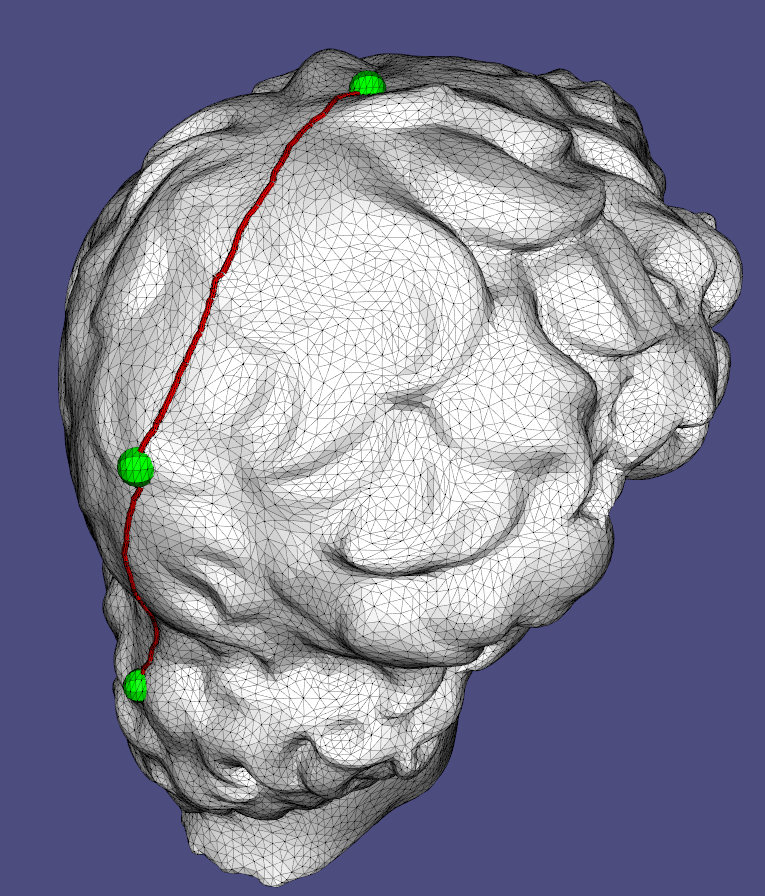
\includegraphics[height=\textwidth]{images/david_euc}
\caption{}
\end{subfigure}
\begin{subfigure}{0.3\textwidth}
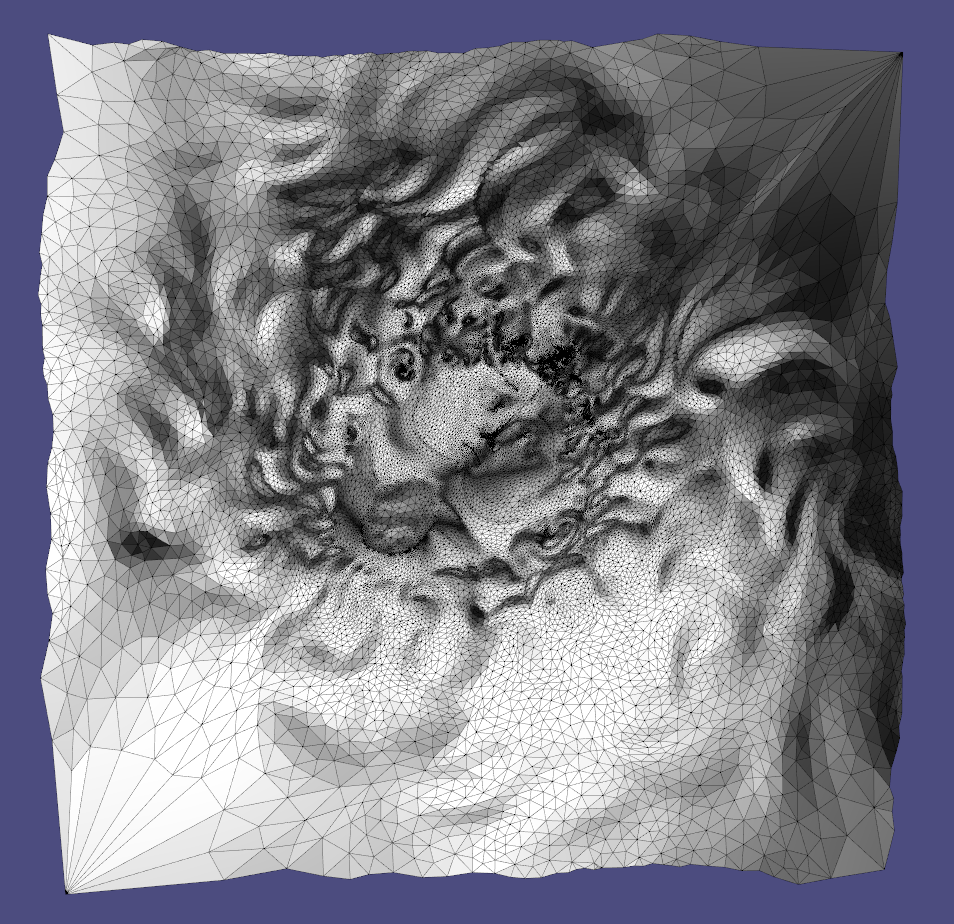
\includegraphics[height=\textwidth]{images/david_euc_emb}
\caption{}
\end{subfigure}\ \ \ \ \ \ \ \ \ \ \ 
\begin{subfigure}{0.3\textwidth}
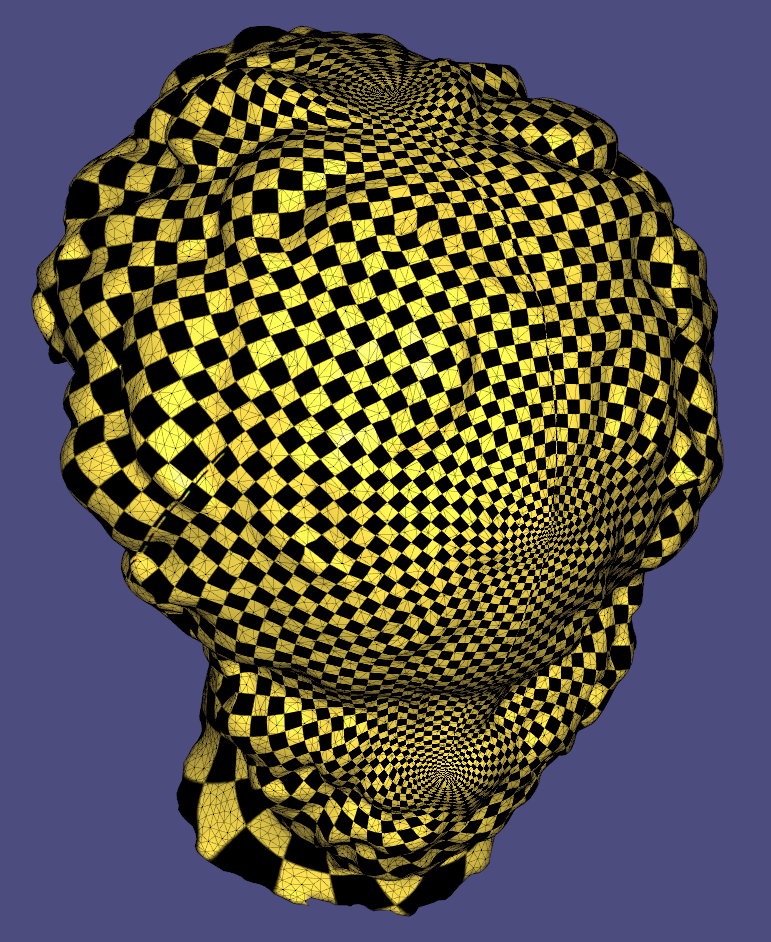
\includegraphics[height=\textwidth]{images/david_euc_texture}
\caption{}
\label{fig:orbifold_conformal}
\end{subfigure}

\begin{subfigure}{0.3\textwidth}
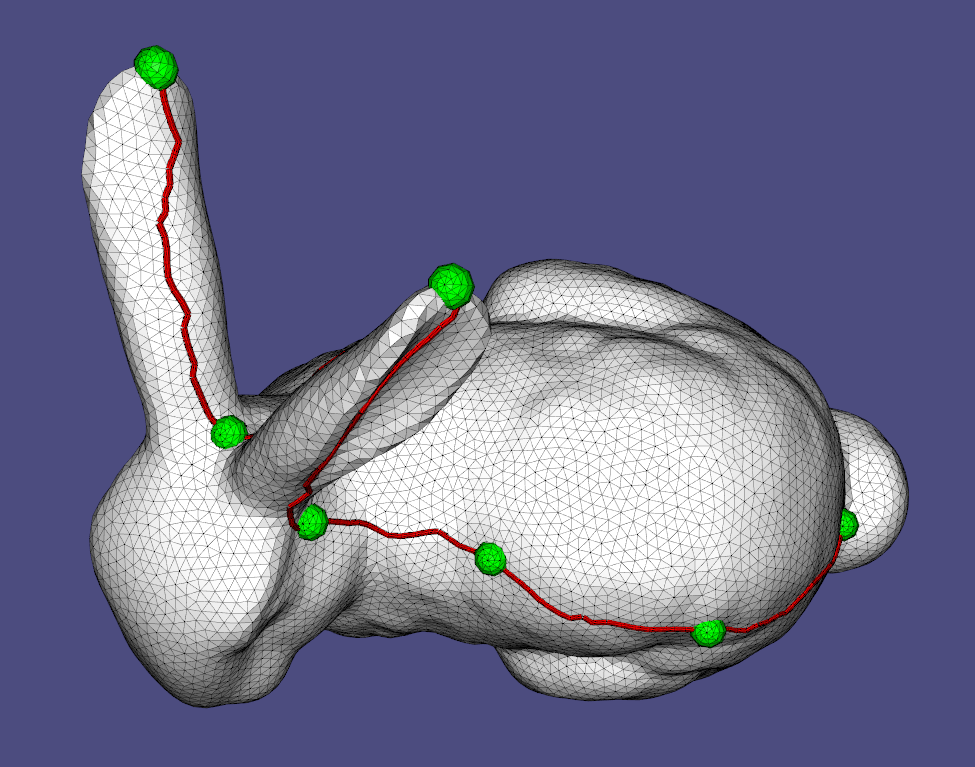
\includegraphics[height=\textwidth]{images/bunny_hyper}
\caption{}
\end{subfigure}\ \ \ \ \ \ \ \ \ \ \ \ \ \ \ \ \ \ \ \ \ \ \ \ \ 
\begin{subfigure}{0.3\textwidth}
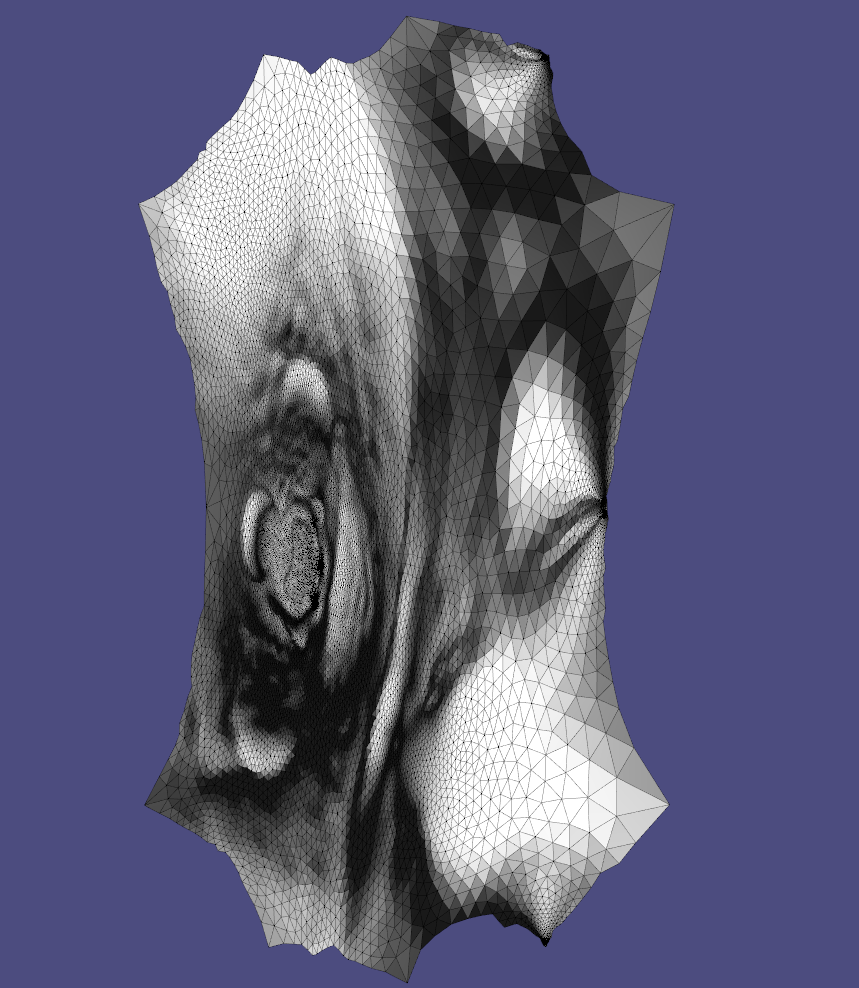
\includegraphics[height=\textwidth]{images/bunny_hyper_emb}
\caption{}
\end{subfigure}
\begin{subfigure}{0.3\textwidth}
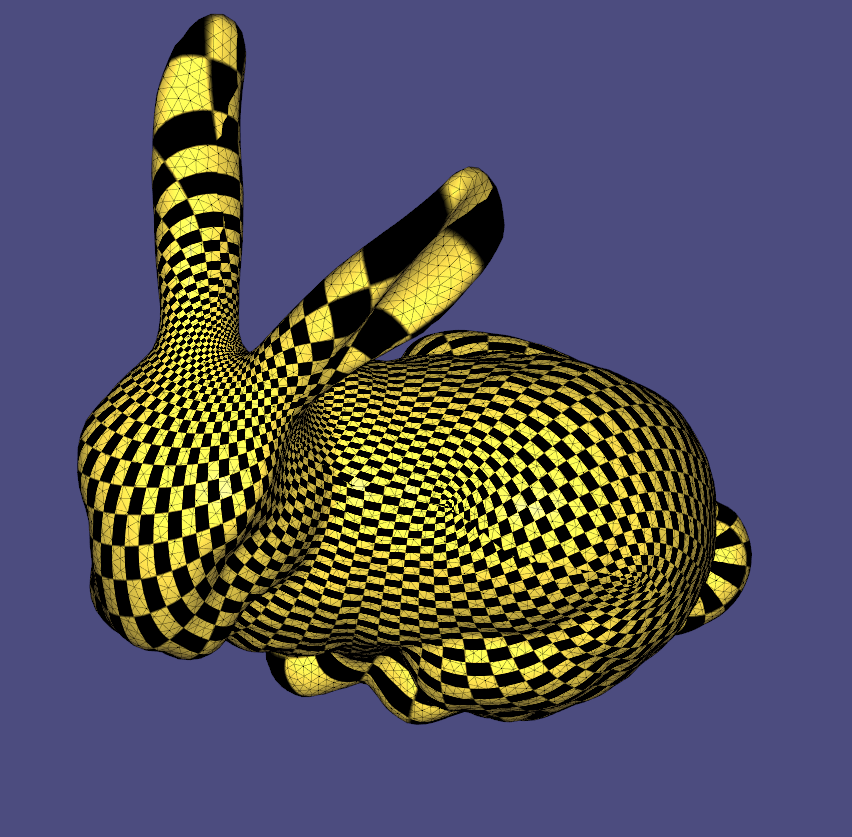
\includegraphics[height=\textwidth]{images/bunny_hyper_texture}
\caption{}
\end{subfigure}
\caption{(a)(d) Models and their cones and slices; (b)(e) Orbifold Tutte embeddings; (c)(f) Texture mappings.}
\label{fig:orbifold_results}
\end{figure}

Note that Euclidean orbifold Tutte embeddings with 3 cones are actually conformal map. It can be seen in Fig.\ref{fig:orbifold_conformal} that the angle are well preserved.



